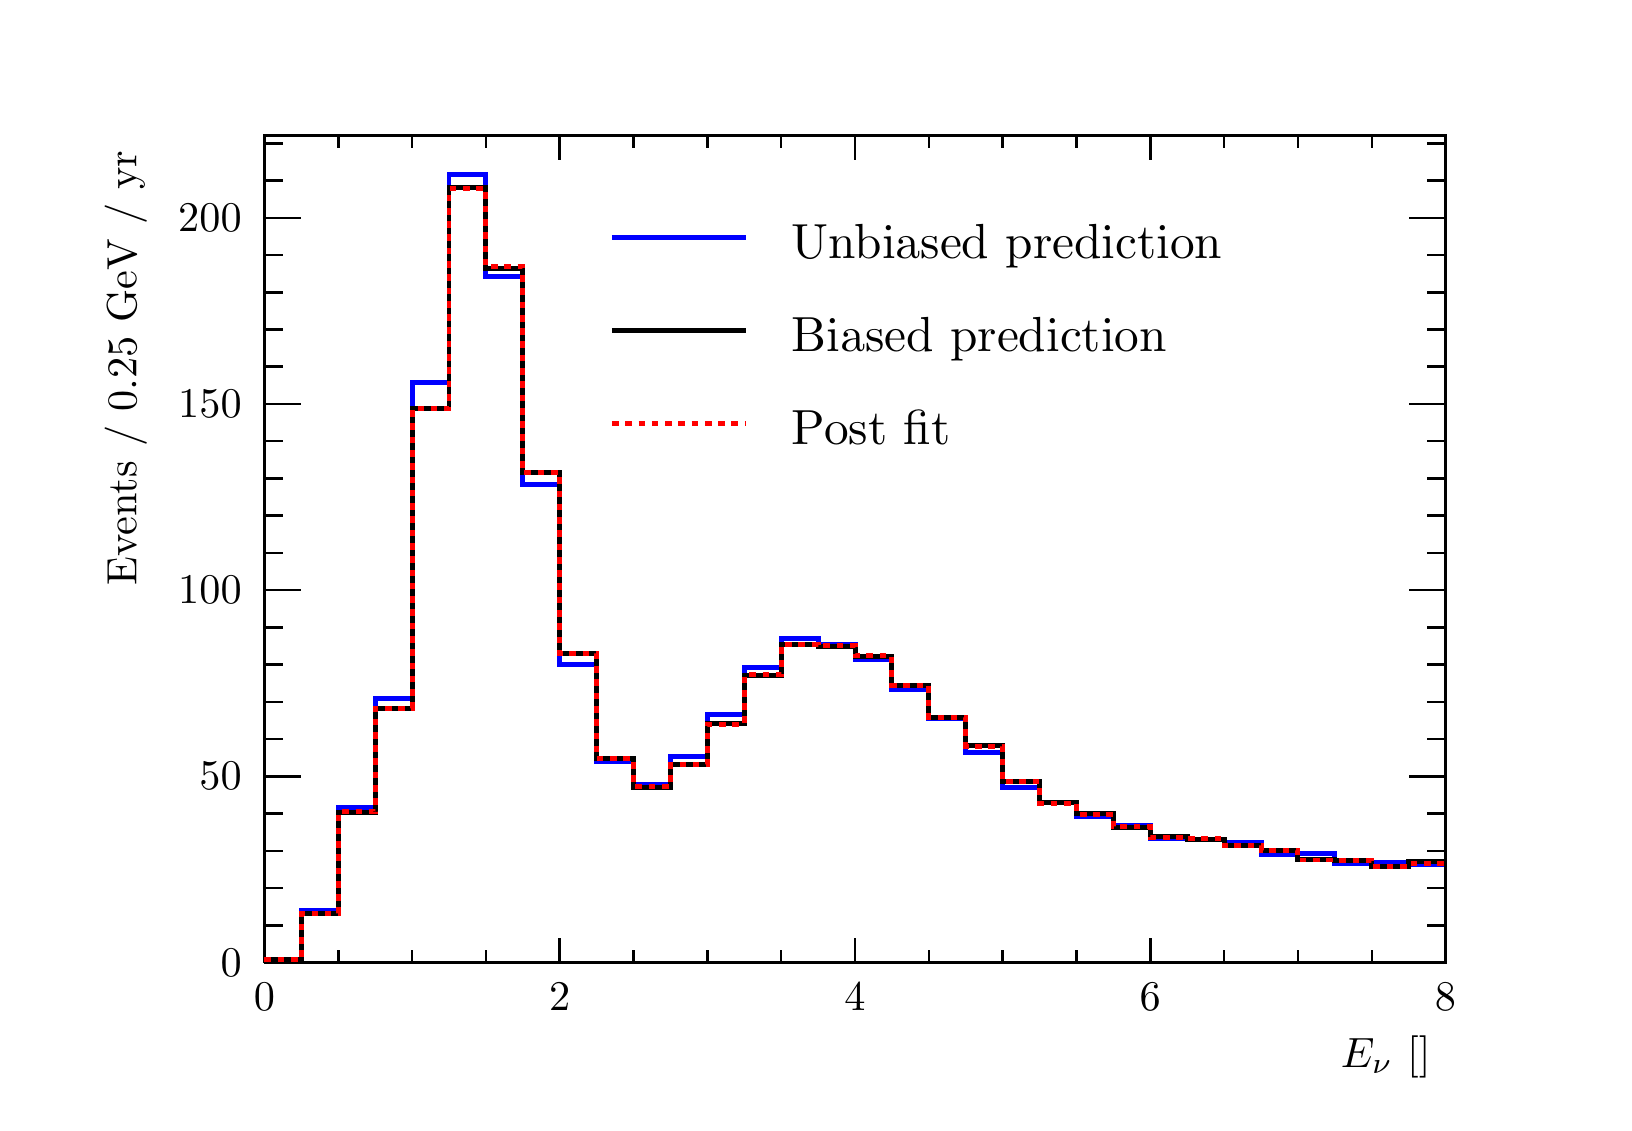
\begin{tikzpicture}
\pgfdeclareplotmark{cross} {
\pgfpathmoveto{\pgfpoint{-0.3\pgfplotmarksize}{\pgfplotmarksize}}
\pgfpathlineto{\pgfpoint{+0.3\pgfplotmarksize}{\pgfplotmarksize}}
\pgfpathlineto{\pgfpoint{+0.3\pgfplotmarksize}{0.3\pgfplotmarksize}}
\pgfpathlineto{\pgfpoint{+1\pgfplotmarksize}{0.3\pgfplotmarksize}}
\pgfpathlineto{\pgfpoint{+1\pgfplotmarksize}{-0.3\pgfplotmarksize}}
\pgfpathlineto{\pgfpoint{+0.3\pgfplotmarksize}{-0.3\pgfplotmarksize}}
\pgfpathlineto{\pgfpoint{+0.3\pgfplotmarksize}{-1.\pgfplotmarksize}}
\pgfpathlineto{\pgfpoint{-0.3\pgfplotmarksize}{-1.\pgfplotmarksize}}
\pgfpathlineto{\pgfpoint{-0.3\pgfplotmarksize}{-0.3\pgfplotmarksize}}
\pgfpathlineto{\pgfpoint{-1.\pgfplotmarksize}{-0.3\pgfplotmarksize}}
\pgfpathlineto{\pgfpoint{-1.\pgfplotmarksize}{0.3\pgfplotmarksize}}
\pgfpathlineto{\pgfpoint{-0.3\pgfplotmarksize}{0.3\pgfplotmarksize}}
\pgfpathclose
\pgfusepathqstroke
}
\pgfdeclareplotmark{cross*} {
\pgfpathmoveto{\pgfpoint{-0.3\pgfplotmarksize}{\pgfplotmarksize}}
\pgfpathlineto{\pgfpoint{+0.3\pgfplotmarksize}{\pgfplotmarksize}}
\pgfpathlineto{\pgfpoint{+0.3\pgfplotmarksize}{0.3\pgfplotmarksize}}
\pgfpathlineto{\pgfpoint{+1\pgfplotmarksize}{0.3\pgfplotmarksize}}
\pgfpathlineto{\pgfpoint{+1\pgfplotmarksize}{-0.3\pgfplotmarksize}}
\pgfpathlineto{\pgfpoint{+0.3\pgfplotmarksize}{-0.3\pgfplotmarksize}}
\pgfpathlineto{\pgfpoint{+0.3\pgfplotmarksize}{-1.\pgfplotmarksize}}
\pgfpathlineto{\pgfpoint{-0.3\pgfplotmarksize}{-1.\pgfplotmarksize}}
\pgfpathlineto{\pgfpoint{-0.3\pgfplotmarksize}{-0.3\pgfplotmarksize}}
\pgfpathlineto{\pgfpoint{-1.\pgfplotmarksize}{-0.3\pgfplotmarksize}}
\pgfpathlineto{\pgfpoint{-1.\pgfplotmarksize}{0.3\pgfplotmarksize}}
\pgfpathlineto{\pgfpoint{-0.3\pgfplotmarksize}{0.3\pgfplotmarksize}}
\pgfpathclose
\pgfusepathqfillstroke
}
\pgfdeclareplotmark{newstar} {
\pgfpathmoveto{\pgfqpoint{0pt}{\pgfplotmarksize}}
\pgfpathlineto{\pgfqpointpolar{44}{0.5\pgfplotmarksize}}
\pgfpathlineto{\pgfqpointpolar{18}{\pgfplotmarksize}}
\pgfpathlineto{\pgfqpointpolar{-20}{0.5\pgfplotmarksize}}
\pgfpathlineto{\pgfqpointpolar{-54}{\pgfplotmarksize}}
\pgfpathlineto{\pgfqpointpolar{-90}{0.5\pgfplotmarksize}}
\pgfpathlineto{\pgfqpointpolar{234}{\pgfplotmarksize}}
\pgfpathlineto{\pgfqpointpolar{198}{0.5\pgfplotmarksize}}
\pgfpathlineto{\pgfqpointpolar{162}{\pgfplotmarksize}}
\pgfpathlineto{\pgfqpointpolar{134}{0.5\pgfplotmarksize}}
\pgfpathclose
\pgfusepathqstroke
}
\pgfdeclareplotmark{newstar*} {
\pgfpathmoveto{\pgfqpoint{0pt}{\pgfplotmarksize}}
\pgfpathlineto{\pgfqpointpolar{44}{0.5\pgfplotmarksize}}
\pgfpathlineto{\pgfqpointpolar{18}{\pgfplotmarksize}}
\pgfpathlineto{\pgfqpointpolar{-20}{0.5\pgfplotmarksize}}
\pgfpathlineto{\pgfqpointpolar{-54}{\pgfplotmarksize}}
\pgfpathlineto{\pgfqpointpolar{-90}{0.5\pgfplotmarksize}}
\pgfpathlineto{\pgfqpointpolar{234}{\pgfplotmarksize}}
\pgfpathlineto{\pgfqpointpolar{198}{0.5\pgfplotmarksize}}
\pgfpathlineto{\pgfqpointpolar{162}{\pgfplotmarksize}}
\pgfpathlineto{\pgfqpointpolar{134}{0.5\pgfplotmarksize}}
\pgfpathclose
\pgfusepathqfillstroke
}
\definecolor{c}{rgb}{1,1,1};
\draw [color=c, fill=c] (0,0) rectangle (20,13.639);
\draw [color=c, fill=c] (3,1.77307) rectangle (18,12.2751);
\definecolor{c}{rgb}{0,0,0};
\draw [c,line width=0.9] (3,1.77307) -- (3,12.2751) -- (18,12.2751) -- (18,1.77307) -- (3,1.77307);
\definecolor{c}{rgb}{1,1,1};
\draw [color=c, fill=c] (3,1.77307) rectangle (18,12.2751);
\definecolor{c}{rgb}{0,0,0};
\draw [c,line width=0.9] (3,1.77307) -- (3,12.2751) -- (18,12.2751) -- (18,1.77307) -- (3,1.77307);
\definecolor{c}{rgb}{0,0,1};
\draw [c,line width=1.8] (3,1.80714) -- (3.46875,1.80714) -- (3.46875,2.42821) -- (3.9375,2.42821) -- (3.9375,3.73615) -- (4.40625,3.73615) -- (4.40625,5.13078) -- (4.875,5.13078) -- (4.875,9.14103) -- (5.34375,9.14103) -- (5.34375,11.775) --
 (5.8125,11.775) -- (5.8125,10.4864) -- (6.28125,10.4864) -- (6.28125,7.84776) -- (6.75,7.84776) -- (6.75,5.56162) -- (7.21875,5.56162) -- (7.21875,4.32291) -- (7.6875,4.32291) -- (7.6875,4.03768) -- (8.15625,4.03768) -- (8.15625,4.38989) --
 (8.625,4.38989) -- (8.625,4.91958) -- (9.09375,4.91958) -- (9.09375,5.52048) -- (9.5625,5.52048) -- (9.5625,5.88942) -- (10.0312,5.88942) -- (10.0312,5.80769) -- (10.5,5.80769) -- (10.5,5.62462) -- (10.9688,5.62462) -- (10.9688,5.24303) --
 (11.4375,5.24303) -- (11.4375,4.87123) -- (11.9062,4.87123) -- (11.9062,4.43668) -- (12.375,4.43668) -- (12.375,4.00024) -- (12.8438,4.00024) -- (12.8438,3.80953) -- (13.3125,3.80953) -- (13.3125,3.63236) -- (13.7812,3.63236) -- (13.7812,3.50747) --
 (14.25,3.50747) -- (14.25,3.35356) -- (14.7188,3.35356) -- (14.7188,3.33532) -- (15.1875,3.33532) -- (15.1875,3.29555) -- (15.6562,3.29555) -- (15.6562,3.14544) -- (16.125,3.14544) -- (16.125,3.1579) -- (16.5938,3.1579) -- (16.5938,3.03099) --
 (17.0625,3.03099) -- (17.0625,3.03761) -- (17.5312,3.03761) -- (17.5312,3.021) -- (18,3.021);
\definecolor{c}{rgb}{0,0,0};
\draw [c,line width=0.9] (3,1.77307) -- (18,1.77307);
\draw [c,line width=0.9] (3,2.07994) -- (3,1.77307);
\draw [c,line width=0.9] (3.9375,1.9265) -- (3.9375,1.77307);
\draw [c,line width=0.9] (4.875,1.9265) -- (4.875,1.77307);
\draw [c,line width=0.9] (5.8125,1.9265) -- (5.8125,1.77307);
\draw [c,line width=0.9] (6.75,2.07994) -- (6.75,1.77307);
\draw [c,line width=0.9] (7.6875,1.9265) -- (7.6875,1.77307);
\draw [c,line width=0.9] (8.625,1.9265) -- (8.625,1.77307);
\draw [c,line width=0.9] (9.5625,1.9265) -- (9.5625,1.77307);
\draw [c,line width=0.9] (10.5,2.07994) -- (10.5,1.77307);
\draw [c,line width=0.9] (11.4375,1.9265) -- (11.4375,1.77307);
\draw [c,line width=0.9] (12.375,1.9265) -- (12.375,1.77307);
\draw [c,line width=0.9] (13.3125,1.9265) -- (13.3125,1.77307);
\draw [c,line width=0.9] (14.25,2.07994) -- (14.25,1.77307);
\draw [c,line width=0.9] (15.1875,1.9265) -- (15.1875,1.77307);
\draw [c,line width=0.9] (16.125,1.9265) -- (16.125,1.77307);
\draw [c,line width=0.9] (17.0625,1.9265) -- (17.0625,1.77307);
\draw [c,line width=0.9] (18,2.07994) -- (18,1.77307);
\draw [anchor=base] (3,1.15931) node[scale=1.52731, color=c, rotate=0]{0};
\draw [anchor=base] (6.75,1.15931) node[scale=1.52731, color=c, rotate=0]{2};
\draw [anchor=base] (10.5,1.15931) node[scale=1.52731, color=c, rotate=0]{4};
\draw [anchor=base] (14.25,1.15931) node[scale=1.52731, color=c, rotate=0]{6};
\draw [anchor=base] (18,1.15931) node[scale=1.52731, color=c, rotate=0]{8};
\draw [anchor= east] (18,0.572837) node[scale=1.52731, color=c, rotate=0]{$E_{\nu}$ [\si{\GeV}]};
\draw [c,line width=0.9] (3,12.2751) -- (18,12.2751);
\draw [c,line width=0.9] (3,11.9682) -- (3,12.2751);
\draw [c,line width=0.9] (3.9375,12.1216) -- (3.9375,12.2751);
\draw [c,line width=0.9] (4.875,12.1216) -- (4.875,12.2751);
\draw [c,line width=0.9] (5.8125,12.1216) -- (5.8125,12.2751);
\draw [c,line width=0.9] (6.75,11.9682) -- (6.75,12.2751);
\draw [c,line width=0.9] (7.6875,12.1216) -- (7.6875,12.2751);
\draw [c,line width=0.9] (8.625,12.1216) -- (8.625,12.2751);
\draw [c,line width=0.9] (9.5625,12.1216) -- (9.5625,12.2751);
\draw [c,line width=0.9] (10.5,11.9682) -- (10.5,12.2751);
\draw [c,line width=0.9] (11.4375,12.1216) -- (11.4375,12.2751);
\draw [c,line width=0.9] (12.375,12.1216) -- (12.375,12.2751);
\draw [c,line width=0.9] (13.3125,12.1216) -- (13.3125,12.2751);
\draw [c,line width=0.9] (14.25,11.9682) -- (14.25,12.2751);
\draw [c,line width=0.9] (15.1875,12.1216) -- (15.1875,12.2751);
\draw [c,line width=0.9] (16.125,12.1216) -- (16.125,12.2751);
\draw [c,line width=0.9] (17.0625,12.1216) -- (17.0625,12.2751);
\draw [c,line width=0.9] (18,11.9682) -- (18,12.2751);
\draw [c,line width=0.9] (3,1.77307) -- (3,12.2751);
\draw [c,line width=0.9] (3.462,1.77307) -- (3,1.77307);
\draw [c,line width=0.9] (3.231,2.24598) -- (3,2.24598);
\draw [c,line width=0.9] (3.231,2.7189) -- (3,2.7189);
\draw [c,line width=0.9] (3.231,3.19182) -- (3,3.19182);
\draw [c,line width=0.9] (3.231,3.66473) -- (3,3.66473);
\draw [c,line width=0.9] (3.462,4.13765) -- (3,4.13765);
\draw [c,line width=0.9] (3.231,4.61057) -- (3,4.61057);
\draw [c,line width=0.9] (3.231,5.08348) -- (3,5.08348);
\draw [c,line width=0.9] (3.231,5.5564) -- (3,5.5564);
\draw [c,line width=0.9] (3.231,6.02932) -- (3,6.02932);
\draw [c,line width=0.9] (3.462,6.50224) -- (3,6.50224);
\draw [c,line width=0.9] (3.231,6.97515) -- (3,6.97515);
\draw [c,line width=0.9] (3.231,7.44807) -- (3,7.44807);
\draw [c,line width=0.9] (3.231,7.92099) -- (3,7.92099);
\draw [c,line width=0.9] (3.231,8.3939) -- (3,8.3939);
\draw [c,line width=0.9] (3.462,8.86682) -- (3,8.86682);
\draw [c,line width=0.9] (3.231,9.33974) -- (3,9.33974);
\draw [c,line width=0.9] (3.231,9.81265) -- (3,9.81265);
\draw [c,line width=0.9] (3.231,10.2856) -- (3,10.2856);
\draw [c,line width=0.9] (3.231,10.7585) -- (3,10.7585);
\draw [c,line width=0.9] (3.462,11.2314) -- (3,11.2314);
\draw [c,line width=0.9] (3.462,11.2314) -- (3,11.2314);
\draw [c,line width=0.9] (3.231,11.7043) -- (3,11.7043);
\draw [c,line width=0.9] (3.231,12.1772) -- (3,12.1772);
\draw [anchor= east] (2.9,1.77307) node[scale=1.52731, color=c, rotate=0]{0};
\draw [anchor= east] (2.9,4.13765) node[scale=1.52731, color=c, rotate=0]{50};
\draw [anchor= east] (2.9,6.50224) node[scale=1.52731, color=c, rotate=0]{100};
\draw [anchor= east] (2.9,8.86682) node[scale=1.52731, color=c, rotate=0]{150};
\draw [anchor= east] (2.9,11.2314) node[scale=1.52731, color=c, rotate=0]{200};
\draw [anchor= east] (1.24,12.2751) node[scale=1.52731, color=c, rotate=90]{Events / 0.25 GeV / yr};
\draw [c,line width=0.9] (18,1.77307) -- (18,12.2751);
\draw [c,line width=0.9] (17.538,1.77307) -- (18,1.77307);
\draw [c,line width=0.9] (17.769,2.24598) -- (18,2.24598);
\draw [c,line width=0.9] (17.769,2.7189) -- (18,2.7189);
\draw [c,line width=0.9] (17.769,3.19182) -- (18,3.19182);
\draw [c,line width=0.9] (17.769,3.66473) -- (18,3.66473);
\draw [c,line width=0.9] (17.538,4.13765) -- (18,4.13765);
\draw [c,line width=0.9] (17.769,4.61057) -- (18,4.61057);
\draw [c,line width=0.9] (17.769,5.08348) -- (18,5.08348);
\draw [c,line width=0.9] (17.769,5.5564) -- (18,5.5564);
\draw [c,line width=0.9] (17.769,6.02932) -- (18,6.02932);
\draw [c,line width=0.9] (17.538,6.50224) -- (18,6.50224);
\draw [c,line width=0.9] (17.769,6.97515) -- (18,6.97515);
\draw [c,line width=0.9] (17.769,7.44807) -- (18,7.44807);
\draw [c,line width=0.9] (17.769,7.92099) -- (18,7.92099);
\draw [c,line width=0.9] (17.769,8.3939) -- (18,8.3939);
\draw [c,line width=0.9] (17.538,8.86682) -- (18,8.86682);
\draw [c,line width=0.9] (17.769,9.33974) -- (18,9.33974);
\draw [c,line width=0.9] (17.769,9.81265) -- (18,9.81265);
\draw [c,line width=0.9] (17.769,10.2856) -- (18,10.2856);
\draw [c,line width=0.9] (17.769,10.7585) -- (18,10.7585);
\draw [c,line width=0.9] (17.538,11.2314) -- (18,11.2314);
\draw [c,line width=0.9] (17.538,11.2314) -- (18,11.2314);
\draw [c,line width=0.9] (17.769,11.7043) -- (18,11.7043);
\draw [c,line width=0.9] (17.769,12.1772) -- (18,12.1772);
\draw [c,line width=1.8] (3,1.80714) -- (3.46875,1.80714) -- (3.46875,2.39373) -- (3.9375,2.39373) -- (3.9375,3.68466) -- (4.40625,3.68466) -- (4.40625,4.99764) -- (4.875,4.99764) -- (4.875,8.8079) -- (5.34375,8.8079) -- (5.34375,11.6155) --
 (5.8125,11.6155) -- (5.8125,10.5871) -- (6.28125,10.5871) -- (6.28125,7.99999) -- (6.75,7.99999) -- (6.75,5.70197) -- (7.21875,5.70197) -- (7.21875,4.36303) -- (7.6875,4.36303) -- (7.6875,3.99054) -- (8.15625,3.99054) -- (8.15625,4.29437) --
 (8.625,4.29437) -- (8.625,4.80614) -- (9.09375,4.80614) -- (9.09375,5.42081) -- (9.5625,5.42081) -- (9.5625,5.81693) -- (10.0312,5.81693) -- (10.0312,5.78823) -- (10.5,5.78823) -- (10.5,5.66545) -- (10.9688,5.66545) -- (10.9688,5.28771) --
 (11.4375,5.28771) -- (11.4375,4.88649) -- (11.9062,4.88649) -- (11.9062,4.52463) -- (12.375,4.52463) -- (12.375,4.07561) -- (12.8438,4.07561) -- (12.8438,3.79974) -- (13.3125,3.79974) -- (13.3125,3.66251) -- (13.7812,3.66251) -- (13.7812,3.48847) --
 (14.25,3.48847) -- (14.25,3.36918) -- (14.7188,3.36918) -- (14.7188,3.33649) -- (15.1875,3.33649) -- (15.1875,3.26517) -- (15.6562,3.26517) -- (15.6562,3.19377) -- (16.125,3.19377) -- (16.125,3.08222) -- (16.5938,3.08222) -- (16.5938,3.07329) --
 (17.0625,3.07329) -- (17.0625,2.98828) -- (17.5312,2.98828) -- (17.5312,3.05882) -- (18,3.05882);
\definecolor{c}{rgb}{1,0,0};
\draw [c,dash pattern=on 2.40pt off 2.40pt ,line width=1.8] (3,1.80716) -- (3.46875,1.80716) -- (3.46875,2.39011) -- (3.9375,2.39011) -- (3.9375,3.6857) -- (4.40625,3.6857) -- (4.40625,5.00135) -- (4.875,5.00135) -- (4.875,8.80365) --
 (5.34375,8.80365) -- (5.34375,11.6006) -- (5.8125,11.6006) -- (5.8125,10.6071) -- (6.28125,10.6071) -- (6.28125,7.99498) -- (6.75,7.99498) -- (6.75,5.69628) -- (7.21875,5.69628) -- (7.21875,4.35848) -- (7.6875,4.35848) -- (7.6875,4.00462) --
 (8.15625,4.00462) -- (8.15625,4.28647) -- (8.625,4.28647) -- (8.625,4.79773) -- (9.09375,4.79773) -- (9.09375,5.42591) -- (9.5625,5.42591) -- (9.5625,5.81606) -- (10.0312,5.81606) -- (10.0312,5.79776) -- (10.5,5.79776) -- (10.5,5.66816) --
 (10.9688,5.66816) -- (10.9688,5.29498) -- (11.4375,5.29498) -- (11.4375,4.88561) -- (11.9062,4.88561) -- (11.9062,4.5202) -- (12.375,4.5202) -- (12.375,4.06902) -- (12.8438,4.06902) -- (12.8438,3.79128) -- (13.3125,3.79128) -- (13.3125,3.65767) --
 (13.7812,3.65767) -- (13.7812,3.49755) -- (14.25,3.49755) -- (14.25,3.36198) -- (14.7188,3.36198) -- (14.7188,3.34247) -- (15.1875,3.34247) -- (15.1875,3.25667) -- (15.6562,3.25667) -- (15.6562,3.19462) -- (16.125,3.19462) -- (16.125,3.07556) --
 (16.5938,3.07556) -- (16.5938,3.07345) -- (17.0625,3.07345) -- (17.0625,2.99853) -- (17.5312,2.99853) -- (17.5312,3.02892) -- (18,3.02892);
\definecolor{c}{rgb}{1,1,1};
\draw [color=c, fill=c] (7.04871,8.02292) rectangle (16.7622,11.5759);
\definecolor{c}{rgb}{0,0,0};
\draw [anchor=base west] (9.47708,10.7173) node[scale=1.78187, color=c, rotate=0]{Unbiased prediction};
\definecolor{c}{rgb}{0,0,1};
\draw [c,line width=1.8] (7.41297,10.9838) -- (9.11282,10.9838);
\definecolor{c}{rgb}{0,0,0};
\draw [anchor=base west] (9.47708,9.53295) node[scale=1.78187, color=c, rotate=0]{Biased prediction};
\draw [c,line width=1.8] (7.41297,9.79943) -- (9.11282,9.79943);
\draw [anchor=base west] (9.47708,8.34861) node[scale=1.78187, color=c, rotate=0]{Post fit};
\definecolor{c}{rgb}{1,0,0};
\draw [c,dash pattern=on 2.40pt off 2.40pt ,line width=1.8] (7.41297,8.61509) -- (9.11282,8.61509);
\end{tikzpicture}
